\section{Architecture}
\label{sec:architecture}

\gate{} is a linear pipeline with strict phase separation
(Figure~\ref{fig:architecture}); each component has a narrow interface,
so the correctness guarantees are maintained by construction rather
than by convention.

\begin{figure}[H]
  \centering
  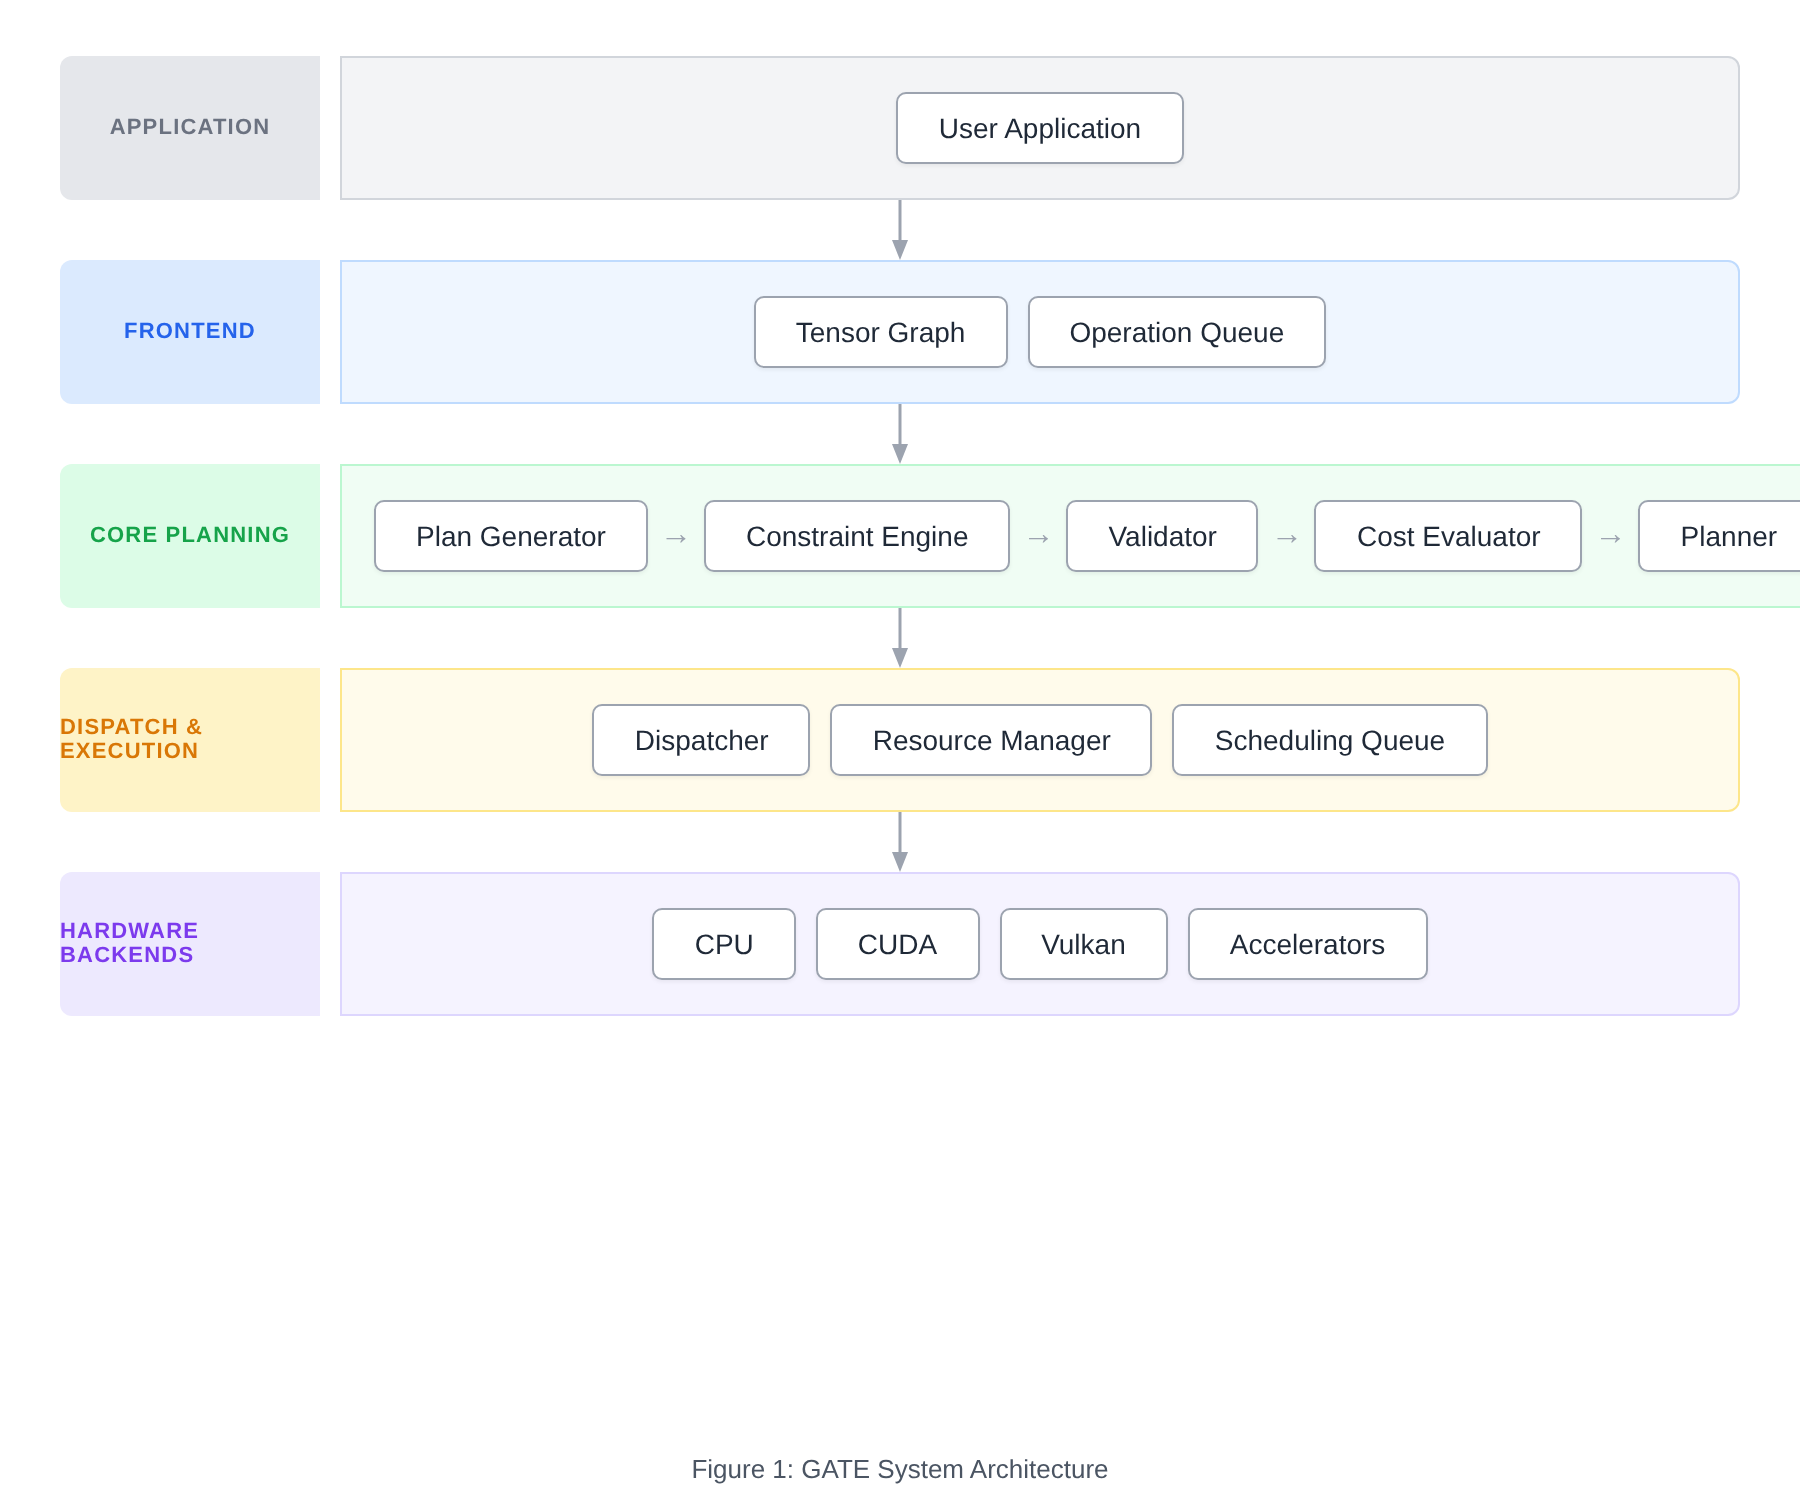
\includegraphics[width=0.92\textwidth]{figures/fig_architecture_diagram.png}
  \caption{High-level \gate{} system architecture.}
  \label{fig:architecture}
\end{figure}

\paragraph{Tensor graph.}
The input IR: a DAG $\mathcal{G} = (V, E)$ of tensor operations and
data dependencies, decoupling front-end model formats (ONNX, GraphDef)
from back-end execution plans. Supports static and symbolic shapes;
immutable during \gate{} execution---all variability lives in the
plans.

\paragraph{Plan generator.}
Produces $\mathcal{P}_{\text{cand}}$ by varying backend assignment,
layout strategy, scheduling order, and fusion decisions; up to $N$
candidates (default 8, max 64), by exhaustive enumeration on small
graphs and heuristic-guided sampling on large ones.

\paragraph{Constraint engine and validator.}
Apply the seven constraint types with early-exit
(Section~\ref{sec:constraint-engine}), producing
$\mathcal{P}_{\text{valid}}$ plus per-rejection diagnostics.

\paragraph{Cost evaluation.}
Computes $\mathbf{m}(P)$ and $\mathcal{C}(P, \mathbf{w})$ for valid
plans only; stateless and safely concurrent.

\paragraph{Planner.}
The orchestration component implementing
Algorithm~\ref{alg:gate}; returns \texttt{ConstraintViolation} with
diagnostics when no valid plan exists.

\paragraph{Dispatcher.}
Executes $P^{*}$: allocates device memory per the plan's layout
assignments, schedules kernels, manages transfers between memory
domains, and collects outputs---translating abstract plan operations
into concrete backend API calls.

\paragraph{Backend.}
The hardware abstraction layer: capability queries, memory management,
and operation execution behind one interface. Current implementations:
CPU (glproc), CUDA (glcuda), Vulkan (glvulkan).

\begin{figure}[H]
  \centering
  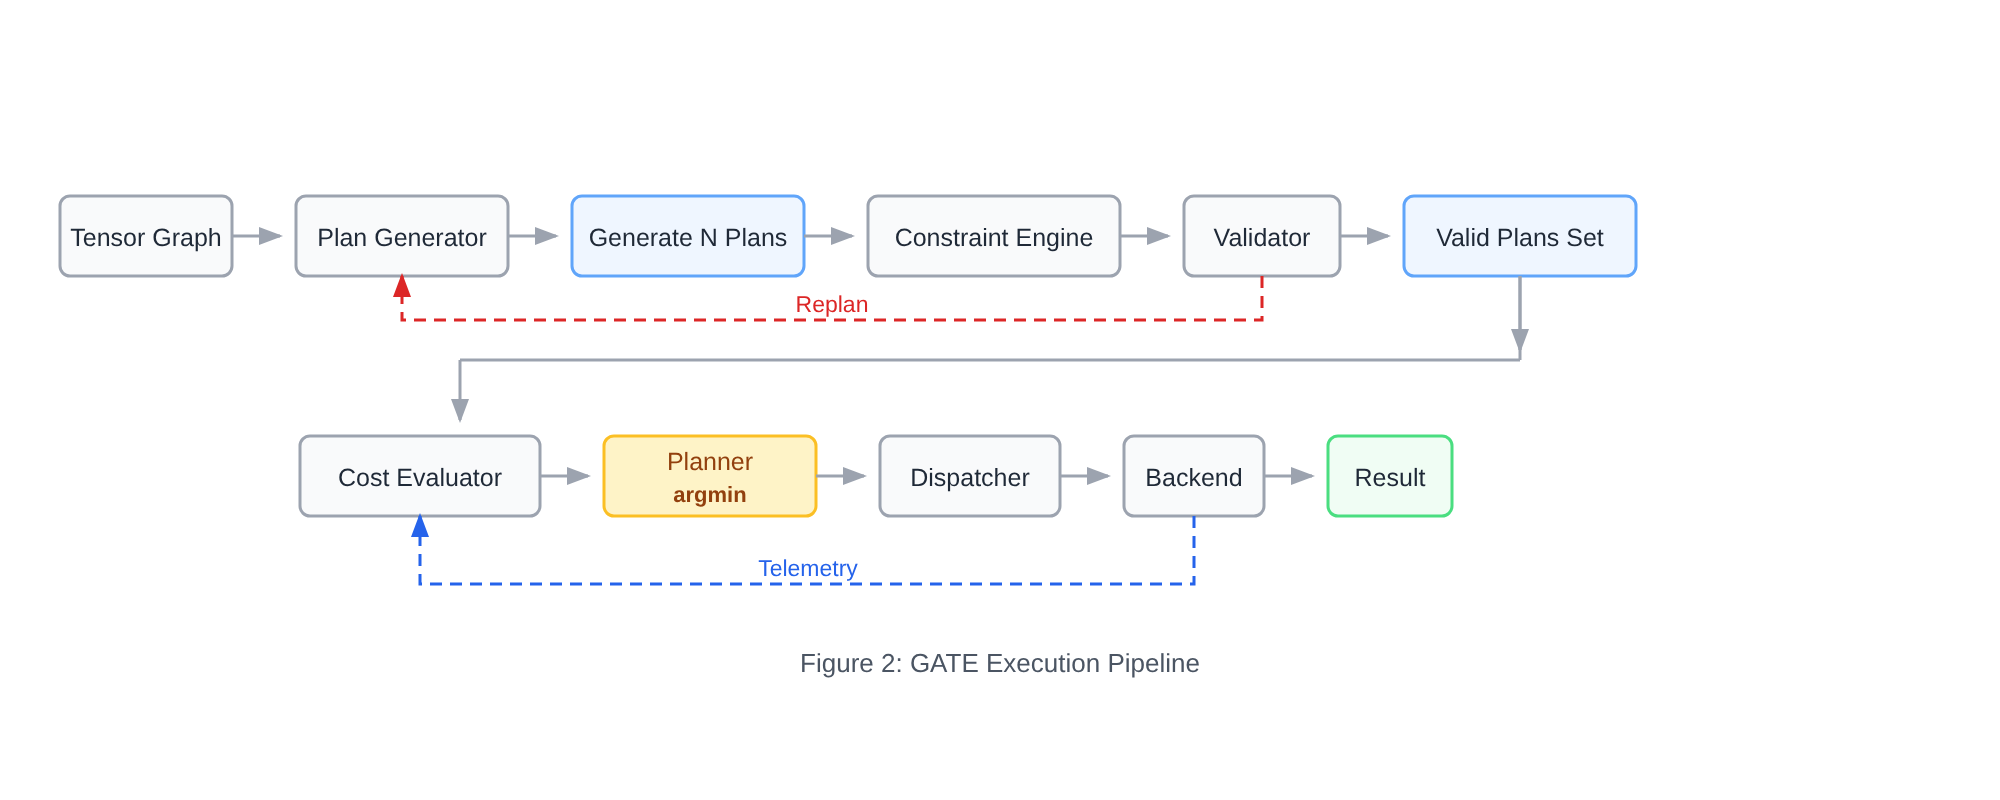
\includegraphics[width=0.92\textwidth]{figures/fig_pipeline_diagram.png}
  \caption{Execution pipeline data flow, generate--validate--evaluate--dispatch.}
  \label{fig:pipeline}
\end{figure}
